\pdfoutput=1
\pdfminorversion=4
\pdfobjcompresslevel=0
% !TeX program = pdflatex
\documentclass[10pt,letterpaper]{article}

\usepackage{txbench-preprint}
\definecolor{todotext}{HTML}{A95F3D}
\newcommand{\todo}[1]{{\color{todotext}\textbf{[TODO:} #1\textbf{]}}}

\preprintKicker{bioRxiv preprint}
\preprintCategory{Computational Biology}
\preprintDate{September 2026}
\preprintTitle{TxBench - Biologics Discovery: Benchmarking AI Agents on Experimentally Grounded Decisions in Therapeutic Antibody Discovery}
\preprintAuthors{Ramesh Ramasamy\preprintSup{1,*}, Hannah Le\preprintSup{1,*}, Jackson Brougher\preprintSup{1,*}, Alex Urrutia\preprintSup{1,*}, Arjun Banerjee\preprintSup{1}, Sean Poust\preprintSup{1}, Kenny Workman\preprintSup{1}}
\preprintAffiliations{\preprintSup{1}LatchBio, San Francisco, CA, USA\\
\preprintSup{*}These authors contributed equally.}
\preprintCorrespondence{kenny@latch.bio}

\begin{document}

\PreprintHeader

\begin{PreprintAbstract}
Biologics discovery requires researchers to integrate heterogeneous experimental evidence and decide whether therapeutic hypotheses, assays, binders, and engineered candidates should advance. We introduce TxBench-Biologics Discovery, a benchmark of 100 experimentally grounded evaluations spanning ten competencies in therapeutic antibody discovery, from target assessment and assay design to cellular pharmacology, engineering, and translational de-risking. Each evaluation is derived from publicly available experimental studies and uses deterministic grading to assess a consequential research decision. Across 17 valid model–harness configurations and three attempts per evaluation, no configuration exceeded a 51\% pass rate; Opus 5 with Claude Code performed best at 50.3\%, followed by Gemini 3.7 Flash with PI at 50.0\%. Failures were often reproducible, although every evaluation was solved by at least one configuration, and 85 were solved by models from at least two families. Model rankings varied across biological competencies, decision types, and evidence sources, while greater cost, token usage, and tool use did not consistently improve accuracy. These results show that current agents remain unreliable at converting experimental evidence into defensible biologics discovery decisions and establish TxBench-Biologics as a framework for evaluating scientific judgment beyond isolated prediction or calculation.
\end{PreprintAbstract}

\vfill
\clearpage


{\fontsize{8.85}{12.0}\selectfont
\newcommand{\TwoColParaBreak}{\par\vspace{0.62em}\noindent}
\noindent\begin{minipage}[t]{0.47\textwidth}
\setlength{\parskip}{0pt}
\setlength{\parindent}{0pt}

\section{Introduction}

Therapeutic biologics discovery is a multiparameter, context-dependent process rather than a sequence of independent assay outcomes. For antibodies, affinity must be considered alongside specificity, stability, solubility, expression, and other properties that ultimately determine whether a molecule can be developed \cite{Jain2017-ye}. Crucially, the meaning of a measurement depends on the experimental system in which it was obtained. Enrichment during phage display, for example, can reflect amplification bias rather than target-dependent selection \cite{Matochko2014-bw}; measurements against purified or solubilized proteins may not fully capture recognition of the target in its native cell-surface context \cite{Lacy2025-do}; and changes in valency or molecular geometry can alter biological activity even when the underlying binding domains remain unchanged \cite{Dickopf2020-to}. Progress through a discovery program therefore depends not simply on identifying the strongest result in a given assay, but on understanding which experiments are informative for the question at hand, how conflicting measurements should be interpreted, and whether the combined evidence supports advancement, redesign, a change in experimental model, or additional experimentation.
\TwoColParaBreak
Existing benchmarks in therapeutic discovery have largely focused on well-defined prediction or design endpoints. Therapeutics Data Commons established standardized datasets and evaluation tasks spanning drug discovery and development \cite{Huang2021-ei}, while antibody-specific resources such as FLAb2 benchmark models against experimentally measured properties including affinity, stability, expression, aggregation, polyreactivity, pharmacokinetics, and immunogenicity \cite{Chungyoun2025-co}. More recently, the AIntibody challenge introduced a prospective, blinded evaluation in which computationally designed antibodies were tested experimentally for affinity and developability \cite{Erasmus2026-qb}. These efforts provide increasingly realistic measures of predictive and design performance, but they generally evaluate a specified molecular property or the quality of a designed candidate. In our prior work, TxBench-PP, we instead evaluated whether AI agents could recover consequential decisions from small-molecule preclinical pharmacology data spanning target engagement, mechanism of action, safety, pharmacokinetics, and translational efficacy \cite{Le2026-tm}. The present benchmark extends this decision-centered approach to biologics discovery, where interpretation often depends on reconciling evidence across molecular format, antigen context, binding, functional activity, and engineering trade-offs.
\TwoColParaBreak
We developed this benchmark to evaluate whether AI systems can make these judgments and turn complex experimental evidence into defensible research decisions. The benchmark focuses on therapeutic antibodies, with tasks grounded in public studies and their underlying experimental data. Each evaluation requires the agent to identify the relevant biological context and comparison, preserve experimental relationships that affect interpretation, reconcile discordant measurements, and distinguish intrinsic molecular properties from effects introduced by assay conditions, selection systems, or engineered formats. The goal is therefore not simply to reproduce an experimental result, but to determine what the available evidence supports and what research action should follow from it.


\end{minipage}\hfill
\begin{minipage}[t]{0.47\textwidth}
\setlength{\parskip}{0pt}
\setlength{\parindent}{0pt}

\section{Benchmark Construction}
We designed the benchmark around a multidimensional set of discovery decisions rather than as a linear collection of assay-specific questions. Its primary axis places each evaluation within the iterative discovery cycle, spanning target and modality selection, experimental design, binder discovery, molecular characterization, functional testing, and subsequent engineering. Additional annotations describe the type of decision, computational approach, therapeutic modality, evidence source, and difficulty. This organization allows performance to be examined across different aspects of discovery judgment without treating any single assay or analytical method as the scientific endpoint. It also reflects the non-linear nature of biologics discovery, where a failure in a functional or native-context assay may require revisiting an earlier decision about the antigen, experimental model, assay design, binder, or therapeutic modality.
\TwoColParaBreak
Evaluations are constructed from public experimental evidence and require agents to determine consequential research actions from the underlying data and experimental design. Related molecules, variants, structures, and studies from the same discovery campaign are assigned to the same benchmark split to limit information leakage across closely related examples. Ground truths are reconstructed from the available data and source methods using analyses that are also available to the agent. Grading is deterministic and assesses the terminal decision together with the supporting quantities or evidence needed to distinguish it from plausible alternatives. Candidate tasks are retained only when the answer is scientifically recoverable, robust to reasonable analytical choices, and distinguishable from plausible but incorrect conclusions. During task development, model rollouts are also examined to separate failures of scientific reasoning from failures caused by formatting, software, or tooling. The resulting unit of evaluation is therefore not an isolated prediction or calculation, but a biologics discovery decision supported by experimental evidence.



\end{minipage}
}

\clearpage

{\fontsize{9.1}{12.8}\selectfont
\section{Benchmark Anatomy}

\begin{multicols}{2}
The benchmark contains 100 evaluations spanning ten competencies across therapeutic biologics discovery (Figure  ~\ref{fig:benchmark-anatomy}). Coverage extends from target opportunity assessment, reagent and assay design, and binder discovery through molecular characterization, cellular pharmacology, engineering, and discovery-stage translational de-risking. The distribution is deliberately broad rather than uniform. Translational de-risking is the largest category, with substantial representation from assay and screening-funnel design, cellular pharmacology, target-hypothesis assessment, and binding characterization. More specialized areas, including binder generation and sequence or lineage analysis, contain fewer evaluations. These counts are intended to describe the scientific breadth of the benchmark, rather than the relative frequency with which these decisions occur in a typical discovery program.
\par
We also classified each evaluation by its primary evidence or analysis substrate and by the type of decision required from the agent. The benchmark includes expression and single-cell data, dose-response and imaging measurements, assay quality-control and hierarchical analyses, binding kinetics, screening and enrichment data, sequence and repertoire information, structural and epitope evidence, and experimental-design problems. Across these settings, the most common decision involves candidate ranking, selection, or triage, followed by experimental design, comparative assessment, mechanistic inference, and integration of multiple lines of evidence into a discovery gate. Other evaluations focus on quantitative characterization or on diagnosing assay and development failures. Together, these complementary classifications show that the benchmark is not dominated by any single assay type or computational procedure. Instead, it tests whether agents can select and apply the appropriate analysis for the specific scientific decision posed at different stages of biologics discovery.

\par
\end{multicols}
}

\begin{center}
  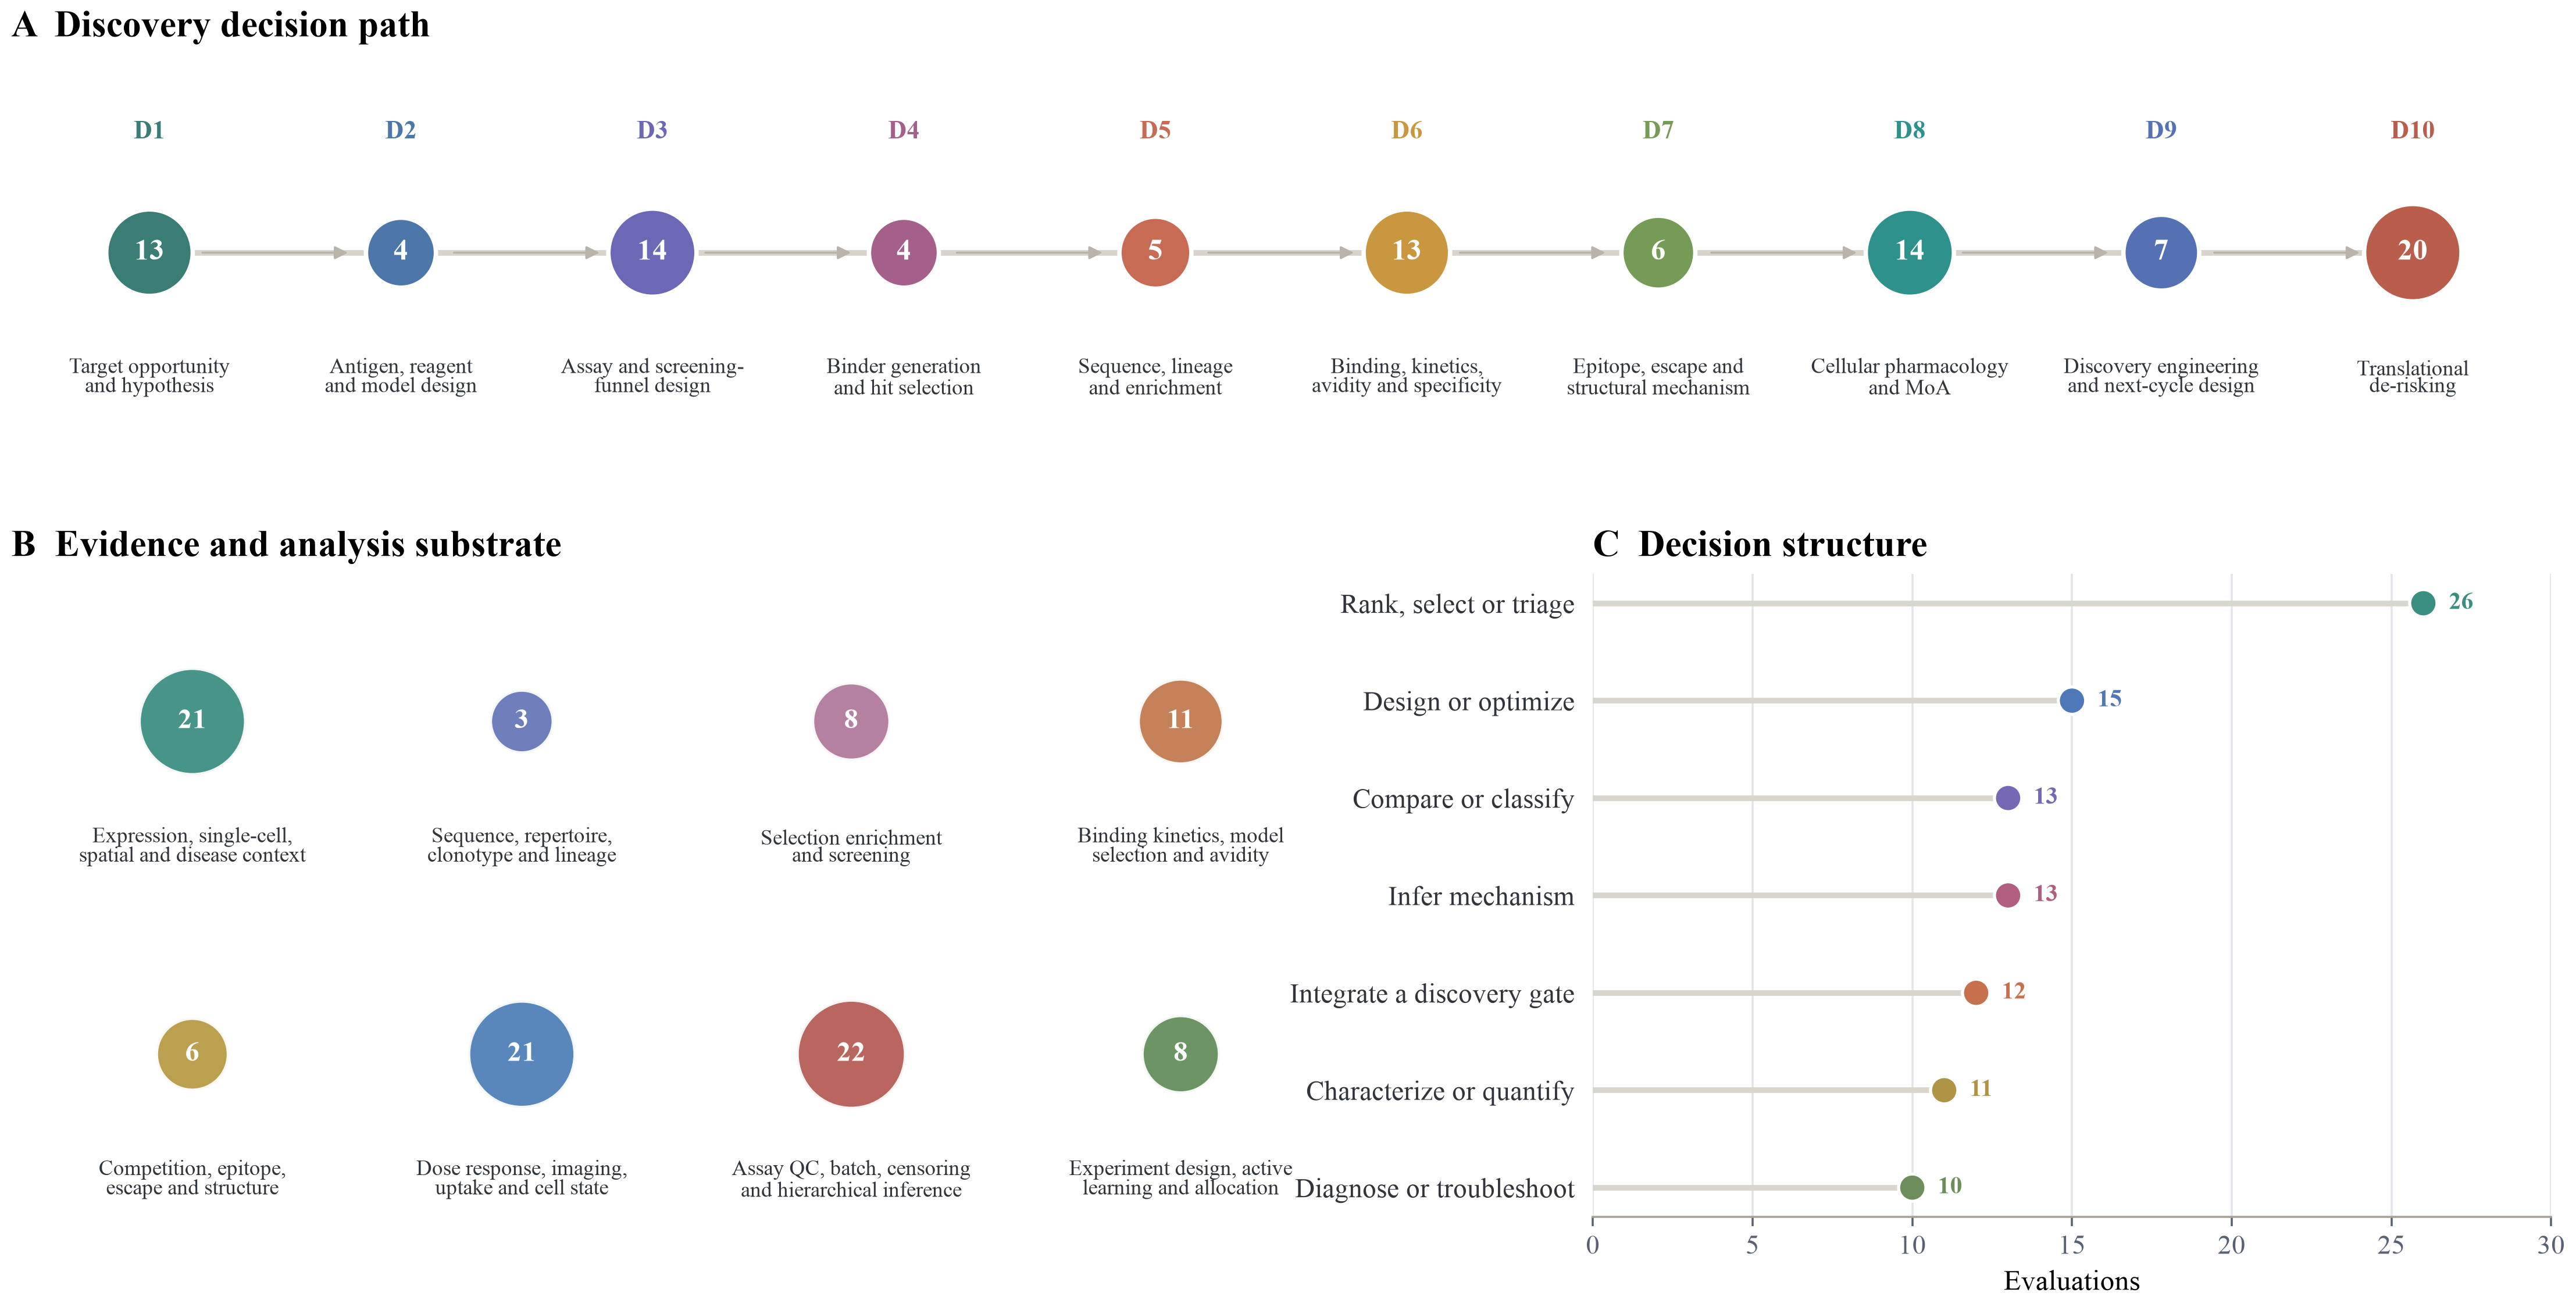
\includegraphics[width=0.96\textwidth]{figures/benchmark_anatomy.png}

  \captionof{figure}{\textbf{Benchmark anatomy.}
 \textbf{A}, Discovery competency labels position evaluations along the therapeutic-biologics discovery path, from target opportunity and experimental design through molecular characterization, cellular pharmacology, engineering, and translational de-risking. Circle area represents the number of evaluations in each category. \textbf{B}, Evidence-and-analysis substrate labels summarize the principal data and analytical families represented in the benchmark; bubble area represents evaluation count. \textbf{C}, Decision-structure labels describe the scientific operation or judgment required for a passing answer; horizontal position indicates evaluation count.}
  \label{fig:benchmark-anatomy}
\end{center}

\StartBody

\section{Results}

\subsection{Even the strongest model–harness configuration failed on nearly half of the evaluations}
We found that no model–harness configuration exceeded a 51\% pass rate, and even the strongest system failed nearly half of all attempts (Figure  ~\ref{fig:leaderboard}). We calculated pass rates on non-refusal attempts and counted execution errors as failures. Opus 5 with Claude Code performed best, passing 151 of 300 attempts (50.3\%). Gemini 3.7 Flash with PI reached a similar pass rate of 50.0\%, followed by Opus 5 with PI at 49.3\%. When we paired the same Gemini 3.7 Flash model with Mini-SWE-Agent, its pass rate fell to 46.0\%, a four-percentage-point difference that indicates a meaningful harness effect even with the underlying model held constant. The OpenAI configurations performed less well overall: GPT-5.6 Sol passed 32.3–33.0\% of attempts across its two harnesses, GPT-5.5 passed 30.7–32.6\%, GPT-5.6 Terra passed 27.7–29.7\%, and GPT-5.6 Luna passed 17.0–18.1\%. Although we observed clear harness effects for some models, differences between underlying models were generally larger.
\par
Performance differences were also highly repeatable at the level of individual evaluations. Among configurations with three non-refused attempts, Opus 5 with Claude Code failed all three attempts on 34 evaluations and passed all three on 36. Gemini 3.7 Flash with PI showed a similar pattern, failing all attempts on 35 evaluations and passing all attempts on 37. Lower-performing models had substantially larger sets of consistently failed evaluations: GPT-5.6 Sol failed all three attempts on 48–49 evaluations, while GPT-5.6 Luna did so on 65–70. Mixed outcomes, in which a configuration passed only one or two of three attempts, were less common than evaluations that were solved or failed consistently. Solvability was mostly reproducible rather than reliant on isolated successes: 91 evaluations were successfully completed at least twice in three attempts by some configuration, 77 were passed in all three attempts by at least one configuration, and 85 were solved by models from at least two independent model families. Aggregate performance differences therefore appear to arise primarily from systematic strengths and weaknesses on particular scientific problems, rather than from isolated stochastic errors.
\EndBody

\begin{center}
  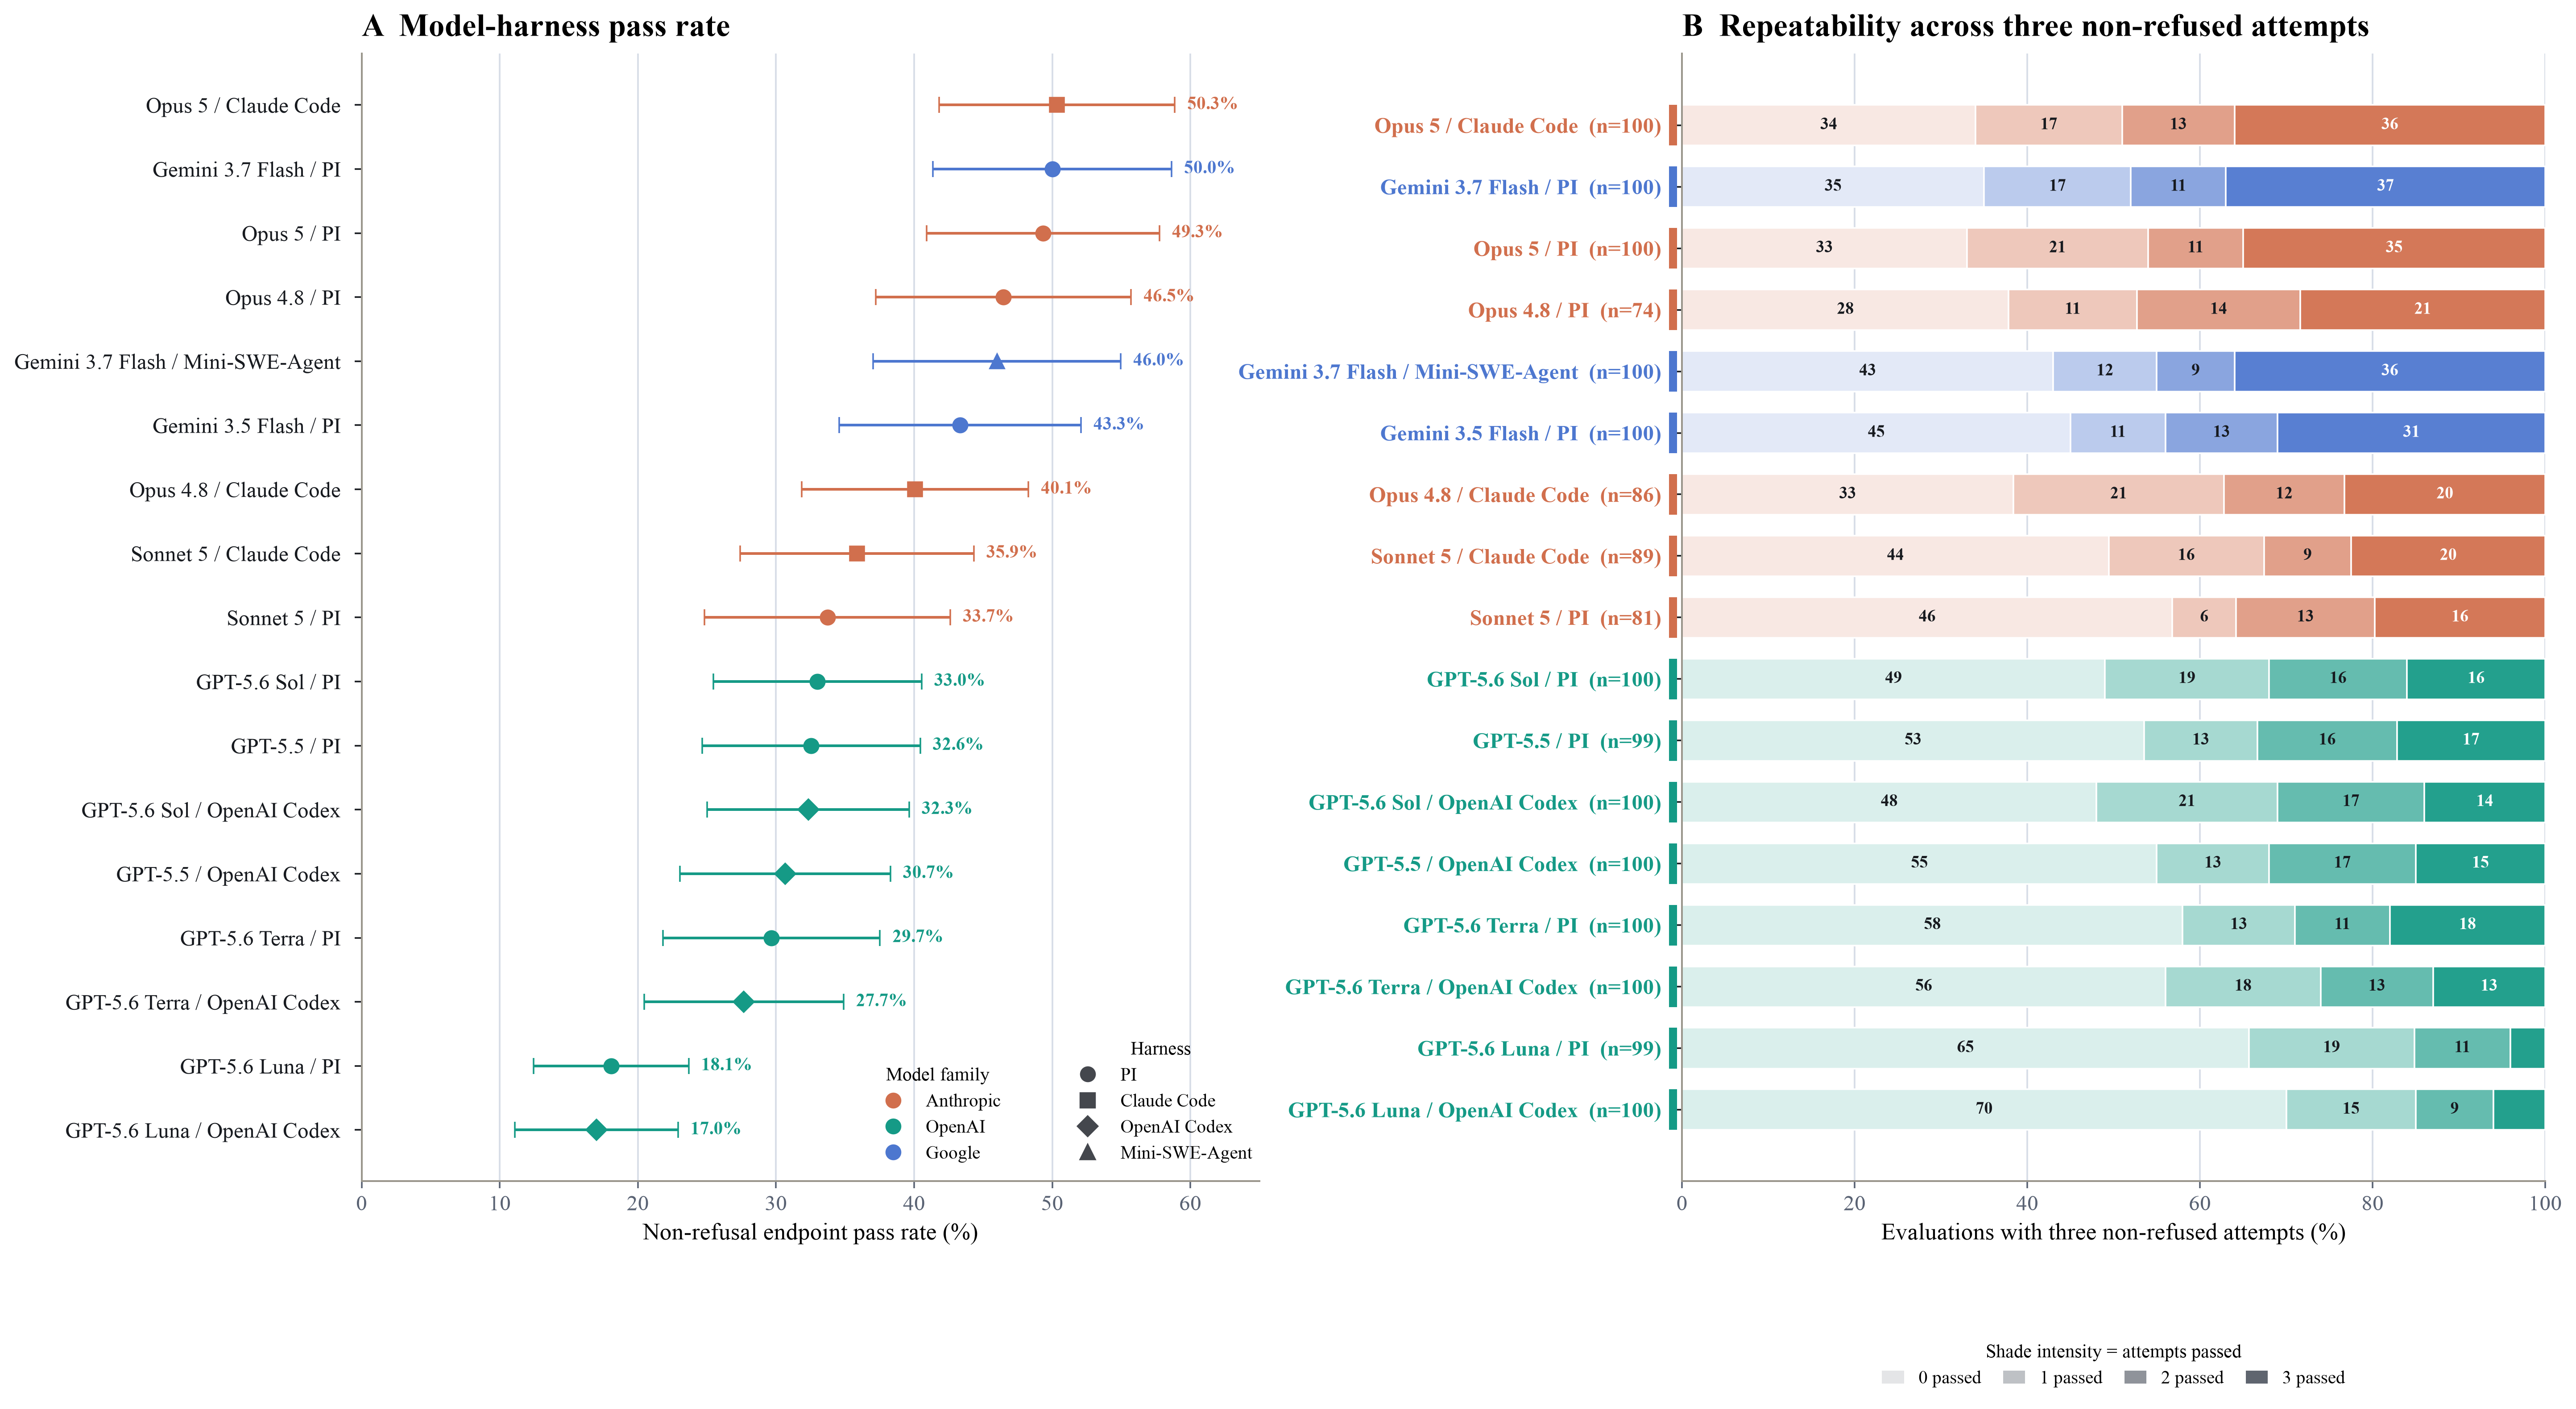
\includegraphics[width=0.96\textwidth]{figures/model_harness_pass_rate_and_repeatability.png}

  \captionof{figure}{\textbf{Model–harness performance and repeatability across TxBench-Biologics.}
  \textbf{A}, Pass rate for each model–harness configuration across 100 evaluations, with three attempts per evaluation. Error bars indicate 95\% Student’s t intervals calculated across per-evaluation pass rates. Colors indicate model family and marker shapes indicate execution harness. \textbf{B}, Evaluation-level consistency across repeated attempts. Analysis was restricted to evaluations with three non-refused attempts for each configuration. Bars are normalized within configuration, with shading from light to dark indicating zero, one, two, or three successful attempts. Numbers within each segment indicate the corresponding evaluation count, and n denotes the number of evaluations with complete non-refused triplicates. Configurations are ordered by their pass rate in panel A.}
  \label{fig:leaderboard}
\end{center}

\ResumeBody
\subsection{More computation does not consistently improve scientific performance}
We observed substantial variation across model–harness configurations in monetary cost, token usage, and tool calls. However, allocating more resources did not consistently improve benchmark performance (Figure  ~\ref{fig:resource-usage}). Opus 5 paired with Claude Code achieved the highest pass rate (50.3\%), averaging approximately \$1.68, 1.10 million tokens, and 21 tool calls per completed run. Gemini 3.7 Flash with PI reached a nearly identical pass rate (50.0\%) at less than one-third the cost (\$0.46 per run), while using substantially more tokens and tools, averaging 1.84 million tokens and 36 tool calls. When we paired the same Gemini model with Mini-SWE-Agent, resource use decreased to \$0.33, 1.10 million tokens, and 25 tool calls per run, but the pass rate also dropped to 46.0\%. We therefore found that similar performance levels could arise from very different execution profiles, and that the choice of harness affected both resource use and observed model performance.
\par
We also found that lower resource use did not necessarily translate to greater efficiency. GPT-5.6 Sol used only 0.43–0.55 million tokens and 15–16 tool calls per completed run, yet passed only 32.3–33.0\% of attempts. GPT-5.6 Luna was the least expensive configuration, at approximately \$0.06 per run, but it produced the lowest pass rates despite relatively high token usage. Conversely, the most expensive configurations did not consistently outperform cheaper alternatives. Gemini 3.7 Flash with PI matched the accuracy of the top-performing Opus 5 configuration at substantially lower cost, while Opus 5 achieved the highest absolute pass rate with fewer tokens and tool calls. These comparisons suggest that cost, token usage, and tool activity capture different aspects of agent execution and should not be treated as interchangeable measures of efficiency.
\par
To understand why additional computation did not always improve performance, we manually examined individual execution trajectories. In a cross-species receptor-translation evaluation (GitHub release URL), Opus 5 with Claude Code passed all three attempts, averaging about 0.29 million tokens and nine tool calls. In each successful trajectory, the model used the measured transcriptional response to identify an inconsistency in the treatment record, reconstruct the correct experimental arms, and calculate the required receptor-chain ratios. Gemini 3.7 Flash with PI failed all three attempts despite using more than twice as many tokens (about 0.63 million) and three times as many tool calls (averaging 27). The model recognized the same inconsistency but retained the incorrect arm assignment, which reversed the relevant expression contrast. Its subsequent calculations then propagated this initial error rather than correcting it. We observed similar behavior in other trajectories: additional computation was useful when it resolved a specific uncertainty in the evidence, but it could also extend an analysis built around an incorrect comparison, estimand, or biological interpretation. Taken together, these results show that resource consumption measures how much work an agent performs, but not whether that work leads to the correct scientific decision.
\EndBody

\begin{center}
  
\includegraphics[width=0.94\textwidth]{paper/figures/model_harness_efficiency.png}

  \captionof{figure}{\textbf{Benchmark performance relative to computational cost, token usage, and tool utilization.} \textbf{A}, Non-refusal endpoint pass rate plotted against the mean monetary cost per completed run. \textbf{B}, Pass rate plotted against the mean total token usage per completed run. The cost and token axes are on logarithmic scales; dashed lines connect configurations along the corresponding accuracy–resource frontier. \textbf{C}, Pass rate plotted against the mean number of tool calls per completed run. Each data point represents a unique model–harness configuration. Point numbers indicate the configuration’s rank by pass rate; colors denote the model family; and marker shapes signify the execution harness. We calculated pass rates across 100 evaluations, with three attempts per evaluation. We excluded model refusals from the analysis, while scoring execution errors as unsuccessful attempts. We averaged resource metrics over completed, non-refused runs that yielded recoverable usage records.}
  \label{fig:resource-usage}
\end{center}

\ResumeBody

\subsection{Model rankings changed across biologics discovery competencies}

We found substantial variation in performance across the ten biologics discovery competencies, and the overall model ranking did not hold consistently across categories (Figure~\ref{fig:by-stage}).
Assay and screening were difficult for all three leading model families, with pass rates of 26.2\% for Opus 5, 40.5\% for Gemini 3.7 Flash, and 21.4\% for GPT-5.6 Sol. These tasks tested whether agents could recognize when an experiment did not support the requested conclusion. Examples included identifying that a dose-response curve without a stable maximal response could not yield a reliable potency estimate, distinguishing target-dependent enrichment from clone growth or amplification during display, and recognizing that assays with different biological meanings could not be collapsed into a single candidate ranking. Binding, kinetics, avidity, and specificity were similarly challenging, with pass rates ranging from 30.8\% to 41.0\%. In these evaluations, agents often had to separate intrinsic molecular affinity from the stronger apparent binding produced by bivalent engagement on high-density cell surfaces and then determine whether that avidity advantage was relevant to the intended tissue. Discovery-stage translational de-risking also remained difficult, with pass rates of 39.2–46.7\%. Decisions in this category required agents to integrate plasma exposure, tissue concentration, dosing route, species biology, and pharmacodynamic response, which could lead to different conclusions about whether a candidate should advance.
\par
The models also showed distinct strengths across biological problem types. Opus 5 performed best on target opportunity and therapeutic-hypothesis decisions (70.5\%) and on cellular pharmacology and mechanism of action (67.9\%), compared with 48.7\% and 51.2\% for Gemini 3.7 Flash and approximately 25\% for GPT-5.6 Sol. These evaluations included deciding whether a tissue-restricted receptor deletion in mice supported ligand neutralization or receptor blockade in humans, and determining whether antibody activity was better explained by molecular geometry, valency, or receptor organization than by affinity alone. Gemini 3.7 Flash showed a different pattern, reaching 72.2\% on epitope, escape, and structural-mechanism evaluations, compared with approximately one-third for Opus 5 and GPT-5.6 Sol. Here, success depended on combining competition experiments, mutational scans, escape profiles, and structural evidence while distinguishing directly observed interactions from assemblies or mechanisms that were only modeled.
\par
GPT-5.6 Sol performed best on sequence, lineage, and enrichment analysis (56.7\%) and discovery engineering and next-cycle design (59.5\%). These tasks included reconstructing relationships among antibody sequences or screening populations and deciding how to allocate the next experimental campaign across candidate families, molecular formats, or receptor-binding arms. Taken together, these reversals show that performance in biologics discovery cannot be summarized by a single model ranking. A model that performed well on sequence or structural evidence could still fail when asked whether that evidence supported biological activity in a different molecular format, cellular system, species, or tissue context. We observed some changes in absolute performance across harnesses, but these did not remove the broader differences in biological decision-making between model families.

\subsection{Performance varied with both decision type and evidence source}
We next decomposed performance using two annotations that span the ten discovery competencies: the type of decision required and the primary evidence used to support it (Figure~\ref{fig:by-task-type}). Quantitative characterization was among the most difficult decision types, with pass rates of 20–38\% across the three model families. The challenge was often not the arithmetic itself but identifying the quantity the experiment could legitimately support. Agents had to distinguish systemic exposure from peak concentration, tissue concentration from measurements on bulk lysate, and directly observed assay values from pharmacokinetic quantities inferred beyond the available data. Comparison and classification tasks were similarly difficult, with pass rates of 24–32\%. In these cases, the key step was often determining whether two measurements were comparable given differences in assay design, species, sample matrix, or treatment context. Performance was more similar across models for assay and development diagnosis, where pass rates clustered between 43\% and 45\%.
\par
Tasks that required combining multiple lines of evidence produced a wider range of outcomes. Opus 5 passed 65\% of mechanism-inference evaluations and 71\% of integrated discovery-gate evaluations. These tasks often required linking observations across biological levels, for example, determining whether receptor engagement translated into downstream function or whether tissue exposure, species biology, and pharmacodynamic response together supported advancing a candidate. Gemini 3.7 Flash performed best on ranking and triage tasks at 60\%, compared with 31\% for GPT-5.6 Sol. This decomposition therefore separates two sources of difficulty that are hidden by the broader competency categories: some evaluations were hard because the required decision involved integrating evidence across biological levels, whereas others were hard because the validity of the comparison itself had to be established before any calculation could be interpreted.
\par
We observed a different pattern when evaluations were grouped by their primary evidence source. Opus 5 reached 60\% on expression, single-cell, and spatial data and 61\% on dose-response, imaging, uptake, and cell-state measurements. Gemini 3.7 Flash reached 75\% on selection and enrichment screens and 69\% on competition, epitope, escape, and structural evidence, but only 27\% on binding-kinetic and avidity problems. GPT-5.6 Sol was relatively stronger on sequence and lineage analysis (44\%), assay QC and hierarchical inference (43\%), and experiment allocation (50\%), while reaching only 20\% on dose-response and cellular-state evidence and 24\% on binding kinetics. These results show that benchmark difficulty was shaped not only by where an evaluation fell in the discovery process but also by the form of evidence available and the type of inference that evidence was expected to support.

\EndBody
\begin{center}
  
\includegraphics[width=0.94\textwidth]{paper/figures/roadmap_category_pass_rates.png}

  \captionof{figure}{\textbf{Benchmark performance across biologics discovery competencies.} \textbf{A}, Mean non-refusal pass rate across evaluations assigned to each roadmap category (D1–D10) for Opus 5, Gemini 3.7 Flash, and GPT-5.6 Sol. Values for each model combine its two evaluated harnesses and are averaged at the evaluation level. \textbf{B}, Non-refusal endpoint pass rate for every model–harness configuration within each category; rows are ordered by overall benchmark performance, and row-label colors indicate model family. Numbers in cells are percentages. Category sample sizes are shown beneath each axis. Refusals were excluded from pass-rate denominators. Each configuration was attempted three times per evaluation.}
  \label{fig:by-stage}
\end{center}
\begin{center}
  
\includegraphics[width=0.94\textwidth]{paper/figures/benchmark_additional_axes_pass_rates.png}

  \captionof{figure}{\textbf{Performance varied with both the scientific decision and the evidence substrate.} \textbf{A}, Non-refusal pass rates for Opus 5, Gemini 3.7 Flash, and GPT-5.6 Sol across seven categories of scientific decision. \textbf{B}, Pass rates for the same models across eight categories representing the primary evidence and analysis substrate. Each evaluation was assigned one primary category on each axis. Results for each model are pooled across the two harnesses tested. Cell labels show pass rates, and n indicates the number of evaluations in each category. Each model–harness configuration was run three times per evaluation.}
  \label{fig:by-task-type}
\end{center}


\ResumeBody

\section{Discussion}
Our results show that frontier agents are not yet reliable decision-makers in biologics discovery. The strongest configuration passed 50.3\% of attempts, and failures were often reproducible across the same evaluations. Because every evaluation was solved by at least one configuration, and 85 were solved by models from at least two families, the observed ceiling is unlikely to reflect a uniformly impossible subset. Instead, it points to stable, capability-specific gaps. This extends TxBench-PP from small-molecule preclinical pharmacology to biologics [8] and is consistent with ScienceAgentBench, BixBench, and LABBench2, which report limitations in realistic scientific work \cite{Chen2024-ov, Laurent2026-zk, Mitchener2025-fo}. Strong performance on knowledge, coding, or narrowly specified prediction benchmarks should not be taken as evidence that an agent can reliably recover research decisions.
\par
Model specialization was equally important. Rankings reversed across competencies, decision types, and evidence sources. Similar limitations have emerged in antibody modeling. FLAb2 found that no evaluated model predicted all developability properties or performed consistently across related datasets \cite{Chungyoun2025-co}, while AbBiBench emphasized evaluating affinity in the context of the antibody–antigen complex \cite{Zhao2025-pb}. CHIMERA-Bench tests generalization to unseen epitopes, antigen folds, and temporally held-out targets \cite{Ahmed2026-uq}, and the blinded AIntibody challenge found that success in one antibody-design task often did not transfer to another \cite{Erasmus2026-qb}. Our results extend this pattern from molecular prediction and design to experimental reasoning. A model that handles sequence or structural evidence well may still misinterpret avidity, cellular context, species translation, or a translational gate. Aggregate scores should therefore be accompanied by stratified capability profiles.
\par
Trajectory analysis showed that more computation alone is unlikely to close these gaps. Additional tokens and tool calls helped when they resolved the decisive ambiguity, but often propagated an incorrect comparator or estimand. BioDesignBench similarly traced much of the protein-design agent gap to shallow candidate evaluation and showed that compute-matched, multi-metric evaluation improved performance \cite{Kim2026-cr}. ScienceAgentBench found that greater inference-time computation improved accuracy, but at substantially higher cost and without achieving reliable task completion [10]. These findings motivate harnesses that explicitly check biological scope, comparator validity, contradictory evidence, and decision sufficiency rather than simply allowing longer trajectories. The benchmark remains retrospective, uses public studies, and lacks human baselines and prospective wet-lab outcomes. Future work should include blinded evaluations of unpublished campaigns, expert comparisons, and experimental validation, following AIntibody \cite{Erasmus2026-qb}. Decision-centered benchmarks can complement predictive and generative benchmarks \cite{Huang2021-ei, Chungyoun2025-co, Erasmus2026-qb, Zhao2025-pb, Ahmed2026-uq} by testing whether a model can determine what the evidence supports and what should happen next.

\columnbreak

\section{Methods}

\subsection{Benchmark composition and data}
The Biologics Discovery Benchmark comprised 100 evaluations derived from publicly available experimental studies. Each evaluation included an agent-facing task, deterministic graders, benchmark annotations, references to staged input data, and private notes documenting the scientific decision and the ground-truth rationale. The benchmark primarily covers therapeutic antibodies and includes engineered antibody formats and other protein-based modalities.

Input materials included source-derived tables, sequences, images, and assay outputs. Identifiers that could reveal the answer were blinded, while decision-relevant experimental structure, including dose, time, donor, replicate, batch, and molecular format, was retained. Evaluations were annotated with discovery competency, decision type, computational-analysis family, therapeutic modality, evidence type, difficulty, and primary failure mode. Related evaluations from the same research campaign were grouped to reduce information leakage.

\subsection{Task format and grading}
Agents received a scientific decision question, a structured response schema, and access to the staged data. Tasks generally did not prescribe the analytical workflow, as selecting an appropriate comparison, representation, or method was part of the skill being evaluated.

All evaluations used deterministic grading. Categorical outputs were assessed using exact matches or predicates; set-valued outputs were evaluated with precision and recall against canonical identifiers; and numeric outputs were assessed using task-specific tolerances or admissible ranges. A run passed only if all required checks passed. Missing required fields, invalid structured responses, and unparseable answers were counted as incorrect.

We reconstructed ground truths from the same evidence available to the agent. We checked candidate tasks for scientific recoverability, information leakage, robustness to reasonable analytical choices, and separation between valid approaches and plausible but incorrect alternatives.

\subsection{Agent runs and execution}
Each evaluation was run three times across 22 model-harness configurations, yielding 6,600 runs. Each configuration paired a language model with the execution scaffold that provided its tools and interaction protocol. The evaluated harnesses included Claude Code, PI, Mini-SWE-Agent, OpenAI Codex, and Grok Build.
 
Models were run at their maximum available reasoning-effort setting in isolated environments without internet access. Agents could inspect and analyze only the files staged for the evaluation. Complete trajectories were retained, including model messages, tool calls, execution outputs, and final responses. Token usage, execution time, and estimated cost were recorded when available.

\subsection{Outcome classification and aggregation}
Each run was classified as correct, incorrect, or refused. A run was correct only if every required grader passed. Gradable answers that failed any required check, along with timeouts and execution errors, were classified as incorrect. Infrastructure-level refusals were detected via provider or harness signals, while model-initiated refusals were identified from the recorded trajectories. Tool denials that did not prevent a gradable final answer were not counted as refusals.

Pass rates were calculated from correct and incorrect runs, with refusals reported separately. Configuration-level performance was averaged across evaluations so that each scientific decision contributed equally. Uncertainty was summarized using 95\% Student’s t intervals across per-evaluation pass rates. Resource-use summaries included only completed, non-refused runs. 

\section*{Data availability}

The public TxBench-PP repository is available at
\url{https://github.com/latchbio/}. It contains a subset of
evaluations and trajectories for manual inspection, along with task definitions,
graders, and available data artifacts for those evaluations. Source assay data
are distributed or linked according to the original data licenses and access
terms.

{\fontsize{8.3}{10.7}\selectfont

\bibliographystyle{unsrt}
\bibliography{paperpile}

}
\EndBody

\end{document}
